\documentclass[tikz]{standalone}
\usepackage{tikz}
\usetikzlibrary{calc}


\tikzset {
	block/.style={
		rectangle,
		draw,
		fill=blue!20,
		rounded corners,
		text width=5em,
		text centered,
		minimum height=2em
	}
}


\begin{document}

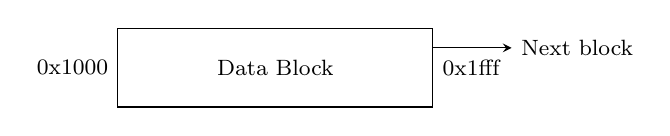
\begin{tikzpicture}[>=stealth, font=\footnotesize]
	\draw (0,0) rectangle (4, 1);
	\node[anchor=east] at (0, 0.5) {0x1000};
	\node[anchor=west] at (4, 0.5) {0x1fff};
	\node at (2, 0.5) {Data Block};

	\draw[->] (4, 0.75) -- +(1,0) node[right] {Next block};
\end{tikzpicture}

\end{document}
